\chapter{定态微扰论}
    理论上讲, 对于任何一个量子力学问题, 我们只要求解出来它的薛定谔方程问题就差不多解决了。但是从$\S$5.2中我们就发现这样做对于绝大多数情况下是不可行的, 比如氢原子我们
    能得到精确解, 但是哪怕是只多了一个电子, 由于相互作用的存在, 我们也无能为力。所以后面要讲的一些近似方法就是在这样的背景下提出来的。如果任何方程都可以很简单的
    找到精确解, 我们也不必要画这么多时间去费力的讨论一些只是近似的处理方法。
    
    这一章要介绍的是\textbf{微扰论(Perturbation theory)}, 经典力学里面天体问题我们也接触过, 那里叫\textbf{摄动法}, 其实英文和微扰是一样的。据说最先是由
    波恩引入量子力学的, 因为他做过一些天体物理, 而那个时候摄动法早就已经广泛的用于天体物理分析了。

    \section{非简并微扰论}
    现在假设对于某个体系, 哈密顿算符为$\hat{H}^0$, 定态薛定谔方程为:
    \begin{equation}
        \label{eq:7.1}
        \hat{H}^0\ket{\psi_n^0}=E_n^0\ket{\psi_n^0}
    \end{equation}
    现在假设对体系做一个小扰动, 哈密顿算符变为:
    \[\hat{H}=\hat{H}^0+\lambda\hat{H}^\prime\quad(\lambda\ll 1)\]
    \begin{thinknote}
    \setlength\parindent{2em}这一点可以这么理解, 比如我们考虑一个无限深势阱, 但是这次势阱的底部“鼓起来了一点”, 我们对于无限深势阱本身是很好求解的, 也就是说对于哈密顿量$\hat{H}^0$,很容易下手,
    对于真实要求解的那个系统, 由于变化不大, 所以说哈密顿量之变化了一个很小的量, 也就是这里的$\hat{H}^\prime$。后面的推导就告诉我们, 这样去做使得我们只需要在原来的无限深势阱模型上
    加上一个小的修正就能达到很好的近似效果了。另外比如说氦原子里面的双电子体系, 我们说过两个电子之间的相互作用会让问题变得极为复杂, 但是如果两个电子之间没有相互作用,
    这个问题就是单纯的两个独立的氢原子问题, 波函数求出来之后求乘积就好。这个时候电子之间的相互作用就可以看作是$\hat{H}^\prime$。
    \end{thinknote}

    显然系统真实的解$\ket{\psi_n}$、$E_n$是和微扰参数$\lambda$有关的, 我们便可以将它们按照$\lambda$的幂级数展开:
    \begin{equation}
        \ket{\psi_n}=\ket{\psi_n^0}+\lambda \ket{\psi_n^1}+\lambda^2\ket{\psi_n^2}+\cdots\\
        E_n=E_n^0+\lambda E_n^1+\lambda^2 E_n^2+\cdots
    \end{equation}
    代入定态薛定谔方程并整理后有\footnote{其实一直到这里数学都很不严谨, 特别是最后还涉及到一个级数之间的求积, 这必须要求级数都绝对收敛。}:
    \begin{equation}
        \label{eq:7.3}
        \begin{aligned}
            &H^0 \ket{\psi_n^0}+\lambda\left(H^0 \ket{\psi_n^1}+H^{\prime} \ket{\psi_n^0}\right)+\lambda^2\left(H^0 \ket{\psi_n^2}+H^{\prime} \ket{\psi_n^1}\right)+\cdots \\
            &\quad=E_n^0 \ket{\psi_n^0}+\lambda\left(E_n^0 \ket{\psi_n^1}+E_n^1 \ket{\psi_n^0}\right)+\lambda^2\left(E_n^0 \ket{\psi_n^2}+E_n^1 \ket{\psi_n^1}+E_n^2 \ket{\psi_n^0}\right)+\cdots
        \end{aligned}
    \end{equation}
    
    根据泰勒展开的唯一性, 我们知道式子两边$\lambda$次数对应相同项要相等。对于$\lambda^0$结果很平凡, 我们现在只考虑一阶修正
    \footnote{\textcolor{red}{特别注意}:我们后面所有的$\hat{H}^\prime$和$E_n^1,E_n^2,\ldots$其实指的都是上面的$\lambda\hat{H}^\prime,\lambda E_n^1,\lambda^2 E_n^2,\ldots$。
    也就是说令$\lambda=1$或者说把这个微扰因子直接吸收进微扰项了。直接说$\lambda=1$可能不太理解, 因为前面提到他是远小于1的, 其实如果你观察的够仔细的话, 我
    们若是直接这么去求, 最后还需要将结果前面乘上$\lambda,\lambda^2,\ldots$这些因子。所以我们还不如就把这些因子提前纳入修正项, 哈密顿算符就直接写成$\hat{H}=\hat{H}^0+\hat{H}^\prime$,对于波函数亦然。
    而前面我们那么写是为了让我们方便理解后面的一阶二阶修正的方程是怎么来的。要是还不理解就想象成麦克劳林级数在1处取值吧。}:
    \begin{equation}
        \label{eq:7.4}
        H^0 \ket{\psi_n^1}+H^{\prime} \ket{\psi_n^0}=E_n^0 \ket{\psi_n^1}+E_n^1 \ket{\psi_n^0}
    \end{equation}
    式子两边左乘$\bra{\psi_n^0}$:
    \[\braket{\psi_n^0|\hat{H}^\prime|\psi_n^0}+\braket{\psi_n^0|\hat{H}^0|\psi_n^1}=E_n^1\braket{\psi_n^0|\psi_n^0}+E_n^0\braket{\psi_n^0|\psi_n^1}\]
    利用态的归一化和下面的连等式(注意到哈密顿算符是厄米算符, 本征值都是实数):
    \[
        \bra{\psi_n^0}\hat{H}^0=\left(\hat{H}^0\ket{\psi_n^0}\right)^\dagger=E_n^0\bra{\psi_n^0}
    \]
    最终得到:
    \begin{lequation}
        \label{eq:7.5}
        \boxed{
            E_n^1=\braket{\psi_n^0|\hat{H}^\prime|\psi_n^0}=\braket{\hat{H}^\prime}_n^0
        }
    \end{lequation}
    
    上面就是很重要的一阶能量修正公式, 我们下一步就是去计算对于波函数的一阶修正。

    首先将\ref{eq:7.4}改写为:
    \begin{equation}
        \label{eq:7.6}
        \left(\hat{H}^0-E_n^0\right)=-\left(\hat{H}^\prime-E_n^1\right)\ket{\psi_n^0}
    \end{equation}
    
    根据上面的推导, 上式右边我们已经完全确定, 所以问题的关键就是再去解上面的这个微分方程。当然, 这也绝非易事, 我们注意到$\{\ket{\psi_n^0}\}$是一个正交完备基\footnote{我们总可以取成这个样子。}
    那么$\ket{\psi_n^1}$实际上就可以在这个基下展开为$\ket{\psi_n^1}=\sum\limits_{m=1}^\infty c_m^{(n)}\ket{\psi_m^0}$, 我们把这个式子代入方程, 便可以充分利用方程的线性简化计算。

    % 下面是早先的版本, 按照格里菲斯的理解方法
    % 在继续之前我们继续做一个简化, 首先注意到$\ket{\psi_n^1}$在$\ket{\psi_n^0}$上的分量完全是任意的。因为如果$\ket{\psi_n^1}$满足方程\ref{eq:7.6}, 
    % 那么$\ket{\psi_n^1}+\alpha\ket{\psi_n^1}$($\alpha$为任意常数)一定也是这个方程的解, 所以我们完全就可以取$c^{(n)}_n=0$, 这样不仅我们多了一个$\braket{\psi_n^0|\psi_n^1}$这样的正交关系, 
    % $\ket{\psi_n^1}$的展开式还简化为:
    % \[\ket{\psi_n^1}=\sum\limits_{m\neq n}^\infty c_m^{(n)}\ket{\psi_m^0}\]
    把这个$\ket{\psi_n^1}$的展开式代入\ref{eq:7.4}并将等式两边左乘$\bra{\psi_\ell^0}$:\footnote{其实这一步是非常容易想到的, 我们其实就是想去求第$\ell$个分量, 而这恰恰就是与基底做内积可以得到的。}\footnote{下面的推导不采用Einstein求和约定。}
    \begin{equation}
        \sum\limits_{m}^\infty c_m^{(n)}\braket{\psi_\ell^0|\hat{H}^0-E_n^0|\psi_m^0}=-\braket{\psi_\ell^0|\hat{H}^\prime-E_n^1|\psi_n^0}
    \end{equation}
    把这个式子展开, 并且注意到$\braket{\psi_\ell^0|\hat{H}^0|\psi_m^0}=E_\ell^0\delta_{m\ell}$, 可以得到:
    \begin{equation}
        c^{(n)}_\ell \left(E^0_\ell -E^0_n\right)\delta_{n\ell}=-\braket{\psi_\ell^0|\hat{H}^\prime-E_n^1|\psi_n^0}
    \end{equation}
    
    对于$n=\ell$的情况, 上面的式子等价于\ref{eq:7.5}, 从中得不到任何有用的信息。
    % \footnote{这不出我们意料, 因为求解前我们就根据方程的性质强制假定了$\ket{\psi_n^0}$方向分量为0}
    现在着重看一下$n\neq\ell$的情况, 直接得出:
    \[c_m^{(n)}=\frac{\braket{\psi_\ell^0|\hat{H}^\prime|\psi_n^0}}{E_n^0-E^0_\ell}\]
    $n=\ell$的情况(也即求解$c_n^{(n)}$)可以根据归一化条件得出:\footnote{这里$\mathcal{O}$表示更高阶的小量, 这里我们只保留到一阶$\braket{\psi_n^1|\psi_n^0}$, $\braket{\psi_n^1|\psi_n^1}$是高一阶的小量}
    \begin{align*}
        1&=\braket{\psi_n|\psi_n}=\braket{\psi_n^0+\psi_n^1+\mathcal{O}|\psi_n^0+\psi_n^1+\mathcal{O}}\\
        &=\underbrace{\braket{\psi_n^0|\psi_n^0}}_{=1}+\left(\braket{\psi_n^0|\psi_n^1}+\braket{\psi_n^1|\psi_n^0}\right)+\mathcal{O}
    \end{align*}
    也即$$\bar{c}_n^{(n)}+c_n^{(n)}=0\Rightarrow c_n^{(n)}=i\gamma\quad\left(\gamma\ll 1\right)$$ 
    也就是说这一项系数是一个\uwave{纯虚数}, 那么考虑一阶修正后的波函数可以写成:
    % \footnote{这里$\lambda c_m^{\prime(n)}\equiv c_m^{(n)}$, 为了下面推导的方便还不能直接取$\lambda=1$, 但最终结果取$\lambda=1$}\footnote{这里第二个等号是因为我们仅考虑到$\mathcal{O}(\lambda)$}
    \begin{align*}
        \ket{\psi_n}&\cong \ket{\psi_n^0}+i\gamma\ket{\psi_n^0}+\sum\limits_{m\neq n}^\infty c_m^{(n)}\ket{\psi_m^0}\\
        &\cong e^{i\gamma\lambda}\ket{\psi_n^0}+\sum\limits_{m\neq n}^\infty c_m^{(n)}\ket{\psi_m^0}
    \end{align*}

    我们说过, 态矢量的相位因子具有任意性, 两个\uwave{成比例}的态之间是不可区分的。那么这里我们给$\ket{\psi_n}$乘上$e^{i\gamma}$不会有任何影响, 不仅消去了零级波函数前面的相位因子, 而且还对第二项在一阶上没有任何影响。
    所以无论$\gamma$的选取如何, 最终得到的$\ket{\psi_n}$都只差了一个相位因子, 没有任何区别。所以我们还不如直接取$\gamma=0$, 这样$\ket{\psi_n^1}$和$\ket{\psi_n^1}$之间还是正交的, 有利于后面的讨论。
    
    综上所述, 波函数的一阶修正便为:
    \begin{lequation}
        \label{eq:7.9}
        \boxed{
            \ket{\psi_n^1}=\sum\limits_{m\neq n}^\infty \frac{\braket{\psi_m^0|\hat{H}^\prime|\psi_n^0}}{E_n^0-E^0_m}\ket{\psi_m^0}
        }
    \end{lequation}
    
    这里问题就出现了, 对于非简并问题, 也就是说\ref{eq:7.1}确定的量子态$\ket{\psi_n^0}$, 不存在能级简并现象, $n \neq m \Leftrightarrow E_n\neq E_m$。
    我们最后得出来的等式就是自洽的。但是一旦能级简并现象存在, 我们这么解就会出现除0问题!这就是我们下一节会讨论的问题。

    最后简要说一下二阶修正, 绝大多数情况下只要考察一阶其实就够了。根据\ref{eq:7.3}:
    \[H^0 \ket{\psi_n^2}+H^{\prime} \ket{\psi_n^1}=E_n^0 \ket{\psi_n^2}+E_n^1 \ket{\psi_n^1}+E_n^2 \ket{\psi_n^0}\]
    跟之前\uwave{一模一样}的推导方法, 我们得到能量的二阶修正项, 那个波函数的修正表达式太dirty了, 之后先用现查(推)吧。
    \begin{lequation}
        \label{eq:7.10}
        E_n^2=\Braket{\psi_n^0|\hat{H}^\prime|\psi_n^1}=\sum\limits_{m\neq n}^\infty\frac{\left|\Braket{\psi_m^0|\hat{H}^\prime|\psi_n^0}\right|^2}{E_n^0-E_m^0}
    \end{lequation}

    现在对\ref{eq:7.9}和\ref{eq:7.10}做一点说明:所谓非简并微扰, 是说我们想去修正的那个$E^0_n$是非简并的, 其它的$E^0_m$可以简并; 我们推导过程中考虑了最简单的情况,
    也就是其它所有$E^0_m$也是简并的, 如果不是, 那么\ref{eq:7.9}和\ref{eq:7.10}中对于$m$求和应该理解为对$E_m^0$的本征子空间$g_m$的所有基矢量求和。

    另外, 其实非简并微扰论还有一个隐含的适用条件就是矩阵元$\braket{\psi_m^0|\hat{H}^\prime|\psi_n^0}$相比于能级间距$\Delta E\equiv E_n^0-E_m^0$是很小的, 否则\ref{eq:7.9}可能不收敛, 
    $E_n^1$给予不了我们任何信息, 这时候就还是要使用简并微扰论了。
    
    最后, 我们来考虑一下一般的物理量$\Omega$的微扰:
    \begin{align*}
        \braket{\hat{\Omega}}&=\Braket{\psi_n|\hat{\Omega}|\psi_n}\\
        &=\left\langle\psi_{n}^{0}|\hat{\Omega}| \psi_{n}^{0}\right\rangle+\lambda\left[\left\langle\psi_{n}^{1}|\hat{\Omega}| \psi_{n}^{0}\right\rangle+\left\langle\psi_{n}^{0}|\hat{\Omega}| \psi_{n}^{1}\right\rangle\right]+\lambda^{2}(\cdots)+\cdots\\
        &\Rightarrow \boxed{\Braket{\hat{\Omega_n}}^1=2\mathrm{Re}\left[\Braket{\psi_n^0|\hat{\Omega}|\psi_n^1}\right]}
    \end{align*}
    再根据\ref{eq:7.9}我们得到:\footnote{显然这里就只适用于非简并微扰论了, 或者说对于非简并微扰, 上式中的$\psi^0$是求出来的零级波函数, 这个情况下非简并微扰与简并微扰后面的计算是如出一辙的}
    \begin{equation}
        \langle\Omega\rangle^{1}=2 \operatorname{Re} \sum_{m \neq n} \frac{\left\langle\psi_{n}^{0}|\hat{\Omega}| \psi_{m}^{0}\right\rangle\left\langle\psi_{m}^{0}\left|H^{\prime}\right| \psi_{n}^{0}\right\rangle}{E_{n}^{0}-E_{m}^{0}}
    \end{equation}
    \section{简并微扰论}
    前面讨论的微扰方法适用的关键是在$\lambda\sim0$时, $\ket{\psi^0}$和$E^0$的变化要很微小,这样$\ket{\psi(\lambda)}$和$E(\lambda)$才能展开成收敛的幂级数形式从而讨论。
    上一节的最后我们也说明了当能级简并出现时, 会出现发散现象。对于无简并情况, 这是显然的, 对应的态在所研究的微扰下变化肯定很小, 否则我们也不会去谈论微扰。
    
    我们先讨论最简单的双重简并情况:
    \[\hat{H}^0\ket{\psi_a^0}=E^0\ket{\psi_a^0},\hat{H}^0\ket{\psi_b^0}=E^0\ket{\psi_b^0}, \braket{\psi_a^0|\psi_b^0}\]
    对于多重简并, 显然对于$\ket{\psi^0}$有无穷多种不同的选择方式:
    \[\ket{\psi^0}=\alpha\ket{\psi_a^0}+\beta\ket{\psi_b^0}\]
    你能确保所有的这些选择都在微扰下变化量很小吗?如果是, 那计算能级微扰就和前面算法一模一样, 但是重点就是我们并非事先能判断出哪个态是我们找寻的进行微扰的态\footnote{后面会介绍一种可直接判断的方法。}。

    下面我们先用一个可以精确求解的例子来说明简并情况下的微扰。
    \begin{thinknote}
        考虑二维简谐振子:
        \[\hat{H}^0=\frac{\hat{p}^2}{2m}+\frac{1}{2}m\left(x^2+y^2\right)\]
        考虑一个存在交叉项的微扰:
        \[\hat{H}^\prime=\epsilon m \omega^2 xy\]
        二维简谐子问题就是两个一维谐振子问题, 我们下面考虑未扰动问题的第一激发态, 这是一个二重简并, 可以取这个子空间的基矢为:
        \begin{align*}
            &\ket{\psi^0}=\ket{\psi^0_0}_x\ket{\psi_1^0}_y=\sqrt{\frac{2}{\pi}}\frac{m\omega}{\hbar}y e^{-\frac{m \omega}{2\hbar}(x^2+y^2)}\\
            &\ket{\psi^0}=\ket{\psi^0_1}_x\ket{\psi_0^0}_y=\sqrt{\frac{2}{\pi}}\frac{m\omega}{\hbar}x e^{-\frac{m \omega}{2\hbar}(x^2+y^2)}
        \end{align*}
        为了精确求解这个问题, 我们作换元:
        \[x=\frac{x^\prime+y^\prime}{\sqrt{2}},y=\frac{x^\prime-y^\prime}{\sqrt{2}}\]
        哈密顿量便可以写为:
        \[\hat{H}=\hat{H}^0+\hat{H}^\prime=\frac{1}{2m}\left(\frac{\partial^2}{\partial^2 x^\prime}+\frac{\partial^2}{\partial^2 y^\prime}\right)+\frac{1}{2}m(1+\epsilon)\omega^2 {x^\prime}^2+\frac{1}{2}m(1-\epsilon)\omega^2{y^\prime}^2\]
        哈密顿量中的二次型化为了标准型, 在这个相当于旋转后的坐标下, 又可以看作是两个独立的简谐振子:
        \[\psi_mn(x^\prime,y^\prime)=\psi^+_m(x^\prime)\psi^-_n(y^\prime),E=\left(m+\frac{1}{2}\right)\omega_+\hbar+\left(n+\frac{1}{2}\right)\omega_-\hbar\]
        上式中的上标$^\pm$标识角频率为$\omega_\pm=\sqrt{1\pm\epsilon}\omega$。

        \setlength\parindent{2em}现在我们重点来看第一激发态, 也即$m+n=1$, 显然随着微扰程度的增大, 简并会慢慢消除为两个能量相差越来越大的两个态(\ref{fig:7.1}的$E_3^0$情形), $\psi_{01}=\psi^+_0(x^\prime)\psi^-_1(y^\prime)$和
        $\psi_{10}=\psi^+_1(x^\prime)\psi^-_0(y^\prime)$。尝试计算下面两个极限:
        \begin{align*}
            &\lim_{\epsilon\to0}\psi_{01}(x,y)=\frac{x-y}{\sqrt{2}}\sqrt{\frac{2}{\pi}}\frac{m\omega}{\hbar} e^{-\frac{m \omega}{2\hbar}(x^2+y^2)}\\
            &\lim_{\epsilon\to0}\psi_{10}(x,y)=\frac{x+y}{\sqrt{2}}\sqrt{\frac{2}{\pi}}\frac{m\omega}{\hbar} e^{-\frac{m \omega}{2\hbar}(x^2+y^2)}
        \end{align*}
        可以发现它们并不等于$\psi^0_a$或是$\psi^0_b$, 而是:
        $$\psi^0(x,y)=\frac{\psi_b^0\pm\psi_a^0}{\sqrt{2}}$$
    \end{thinknote}

    举上面的这个例子是想说明, 未微扰态和微扰态之间是连续变化的, 而因为能级简并, 未微扰态有很多种, 而真正能进行微扰展开的就那几个, 而这些又不是先验的。
    所以我们不能盲目的再像上一节一样直接随便选取一个态做微扰。

    下面这张图展现了体系微扰时可能发生的几种情况, 其中每一条曲线上的一个点都代表一个量子态, 而一条曲线就代表未微扰态到微扰态的连续变化。从图中可以清晰的看到简并的消除以及额外简并的出现($\lambda_1$)。
    \begin{figure}[htbp]
        \centering
        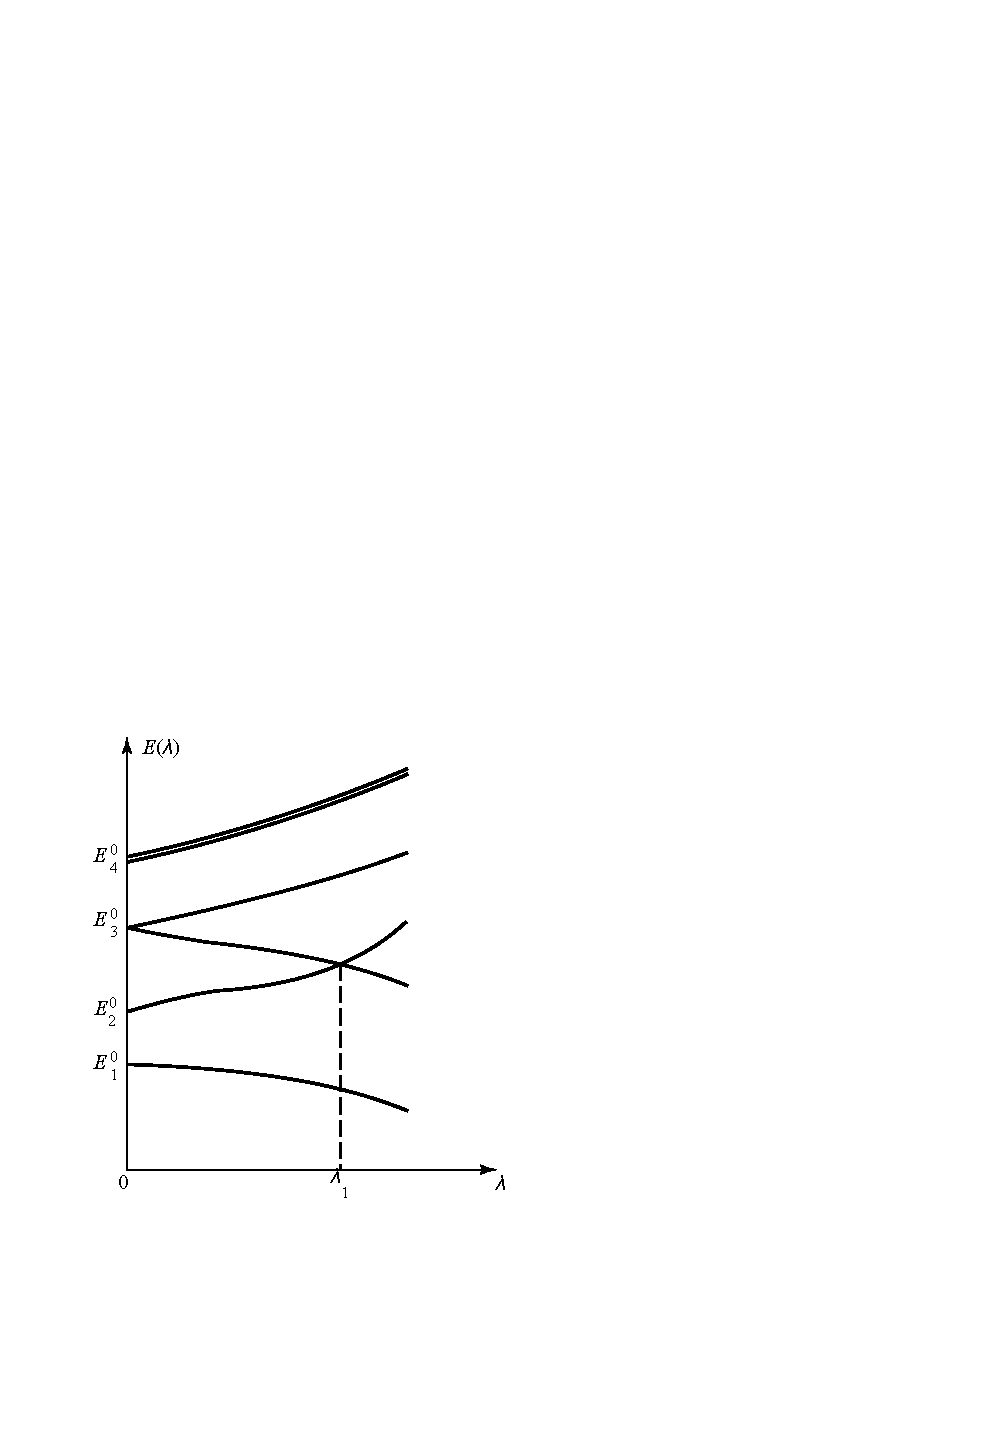
\includegraphics[scale=0.7]{fig/7.1.pdf}
        \caption{简并微扰的多种情况}
        \label{fig:7.1}
    \end{figure} 

    下面我们假设我们已经找到了那个合适的态$\ket{\psi^0}=\alpha\ket{\psi_a^0}+\beta\ket{\psi_b^0}$,其中$\alpha$和$\beta$是待定的。
    
    那么这个时候我们在$\ket{\psi^0}$附近进行微扰展开是合理的, 根据\ref{eq:7.4}, 我们依旧可以得到一阶近似:
    \[H^0 \ket{\psi_n^1}+H^{\prime} \ket{\psi_n^0}=E_n^0 \ket{\psi_n^1}+E_n^1 \ket{\psi_n^0}\]
    还是一样的套路, 这次两边同时左乘$\bra{\psi_a^0}$,得到:
    \[\alpha\braket{\psi_a^0|\hat{H}^\prime|\psi_a^0}+\beta\braket{\psi_a^0|\hat{H}^\prime|\psi_b^0}=E^1 \alpha\]
    同理,两边同时左乘$\bra{\psi_b^0}$,得到:
    \[\alpha\braket{\psi_b^0|\hat{H}^\prime|\psi_a^0}+\beta\braket{\psi_b^0|\hat{H}^\prime|\psi_b^0}=E^1 \beta\]
    我们定义$W_{i j} \equiv\left\langle\psi_{i}^{0}\left|H^{\prime}\right| \psi_{j}^{0}\right\rangle , (i, j=a, b) $, , 我们可以将上面的方程写成矩阵形式:
    \begin{equation}
        {\color{red}
            \underbrace{\left(\begin{array}{ll}
                W_{a a} & W_{a b} \\
                W_{b a} & W_{b b}
                \end{array}\right)}_{\mathrm{W}}\left(\begin{array}{l}
                \alpha \\
                \beta
                \end{array}\right)=E^{1}\left(\begin{array}{c}
                \alpha \\
                \beta
                \end{array}\right) 
        }
    \end{equation}
    
    也就是说, 我们要计算能级的一阶修正, 先在简并态子空间中选取任意一组基底${\ket{\psi_a^0},\ket{\psi_b^0}}$, 然后依次写出$\hat{H}^\prime$的矩阵元, 并
    排列成矩阵$\mathbf{W}$, 它的本征值便是$E^1$, 顺带算出来的本征矢就是$\ket{\psi^0}$。\footnote{但是注意了, 如果计算出来$\mathbf{W}$两个本征值相等, 这个时候依然无法确定$\ket{\psi^0}$, 这个时候就要去认真考虑$\ket{\psi}$的修正了(需要使用高阶简并微扰理论)。好在很多情况下研究能级修正就够了。}
    \begin{equation}
        \boxed{E_{\pm}^{1}=\frac{1}{2}\left[W_{a a}+W_{b b} \pm \sqrt{\left(W_{a a}-W_{b b}\right)^{2}+4\left|W_{a b}\right|^{2}}\right]}
    \end{equation}
    
    如果我们运气很好, $\ket{\psi_a^0}$和$\ket{\psi_b^0}$恰好就是能够在附近直接微扰展开的态, 显然, 它们将$\mathbf{W}$对角化。这个时候会发现
    \[E_{+}^{1}=W_{a a}=\left\langle\psi_{a}^{0}\left|H^{\prime}\right| \psi_{a}^{0}\right\rangle, \quad E_{-}^{1}=W_{b b}=\left\langle\psi_{b}^{0}\left|H^{\prime}\right| \psi_{b}^{0}\right\rangle\]
    这就是我们在非简并情况下的计算公式!也印证了前面说的, 如果选取的$\ket{\psi^0}$合适, 后面的推导和非简并情况是完全一致的。

    从上面的一系列推导来看, 计算能级微扰最简单的方法就是先知晓正确的$\ket{\psi^0}$。 那有没有一种方式, 能在我们没有求解之前, 就能\uwave{猜出}那些合适的$\ket{\psi^0}$?下面这个定理比较常用。
    \begin{theorem}{Good State}
        如果算符$\hat A$与哈密顿算符$\hat{H}^0,\hat{H}^\prime$均对易, $\ket{\psi^0_a}$与$\ket{\psi^0_b}$是$\hat A$与$\hat{H}^0$的共同本征矢, 即:
        \[A \ket{\psi_a^0}=\mu \ket{\psi_a^0}, \quad A \ket{\psi_b^0}=v \ket{\psi_b^0}, \quad {\color{red}\text { and } \mu \neq v}\]
        那么$\ket{\psi_a^0}$和$\ket{\psi_a^0}$就是我们要找的合适的$\ket{\psi^0}$(\textbf{good states})。
    \end{theorem}

    关于这个定理的证明不想说太多, 实际上就是寻找(\uwave{局部的})CSCO的过程。

    那问题又来了, 怎么确定那个$\hat{A}$呢?回忆一下第六章, 讨论系统的对成性, 我们知道每一种对称操作对应一个算符, 宇称算符、平移算符、旋转算符, 而系统具有的每一种对称性又对应其中某一种算符
    与$\hat{H}$的对易性。而系统的对称性我们是可以很直观地通过哈密顿量看出来的。

    \subsection*{多重简并情况}
    这个推广就很显然了, 对于最一般的n重简并的态, 只要先选取一套$\hat{H}^0$对应这个能级的本征子空间正交基。写出对应的$W$矩阵, 然后求其本征值得能级一阶修正, 
    求其本征矢得零级波函数$\ket{\psi^0}$。不同的只是这里我们要处理更复杂的$n\times n$矩阵罢了。
    
    \subsection*{Feynman-Hellmann 定理}
    \begin{theorem}{Feynman-Hellmann 定理}
        如果哈密顿量$\hat{H}(\lambda)$依赖于某个参数$\lambda$, 那么\textbf{定态波函数}$\psi_n(\lambda)$和对应的能级$E_n(\lambda)$都会依赖于$\lambda$, 而且有下面等式成立:
        \begin{equation}
            \label{eq:fht}
            \frac{dE_n}{d\lambda}=\Braket{\psi_n|\frac{d\hat{H}}{d\lambda}|\psi_n}
        \end{equation}
        其中$E_n$这一能级是不简并的, 或者简并, 但是$\psi_n$为$\lambda$微扰时的零级波函数。
    \end{theorem}
    
    此定理有很多种不同的证明方式, 实际上根据前面学的微扰论可以作如下证明:
    \begin{thinknote}
        \textbf{Proof}:

            \begin{equation*}
                \hat{H}(\lambda+\Delta\lambda)=\hat{H}(\lambda)+\frac{d\hat{H}}{d\lambda}\Delta\lambda+\mathcal{O}(\Delta\lambda)
            \end{equation*}
            我们便可以通过微扰论得到能量的一阶修正:
            \begin{equation*}
                E_n^\prime=E_n+\Braket{\psi_n|\frac{d\hat{H}}{d\lambda}|\psi_n}\Delta\lambda+\mathcal{O}(\Delta\lambda)
            \end{equation*}
            上面的式子也等价于
            \begin{equation*}
                \Delta E_n=\Braket{\psi_n|\frac{d\hat{H}}{d\lambda}|\psi_n}\Delta\lambda+\mathcal{O}(\Delta\lambda)
            \end{equation*}
            我们把上式两边同时除以$\Delta\lambda$, 再取$\Delta\lambda\to 0$的极限便得到了\ref{eq:fht}。
    \end{thinknote}

    \section{氢原子的精细结构}
    第四章中我们详细考虑过氢原子的能级问题, 而且指出每个能级的简并态有$n^2$个。但实际上不是这样的, 首先由于质子并不是不“动”的, 所以实际上我们需要把能级公式中的
    $m_e$换成约化质量$\mu$, 但是这个问题很trivial, 修正量很小, 而且并不会引发能级消除, 也即改变能级结构。我们重点考虑的是其它效应, 首先说明, 我们下面的所有计算其实
    在相对论量子力学中(利用Dirac方程)都可以严格求解。

    在行星公转问题中, 比如著名的水星近日点偏移效应, 就是同时考虑了广义和狭义相对论的修正结果。同样在量子力学中, 我们也有相对论修正, 但是我们只考虑狭义相对论。
    
    未考虑修正的氢原子能谱称为\textbf{玻尔能级(Bohr energies)};考虑了狭义相对论效应和电子自旋轨道耦合效应共同的修正称为\textbf{氢原子的精细结构(Fine structure)};
    进一步考虑电磁场的量子化效应的修正后称为\textbf{兰姆移位(Lamb shift)};更进一步考虑电子与质子之间的偶极矩的磁相互作用后称为\textbf{超精细结构(hyperfine structure)}。
    
    我们定义氢原子的精细结构常数:
    \begin{equation}
        \boxed{\alpha\equiv\frac{e^2}{4\pi \epsilon_0\hbar c}\approx\frac{1}{137.036}}
    \end{equation}
    下面这张表总结了不同效应带来的修正的数量级:
    \begin{center}
        \begin{tabular}{|rll|}
            \hline Bohr energies: & of order & $\alpha^2 m_e c^2$ \\
            Fine structure: & of order & $\alpha^4 m_e c^2$ \\
            Lamb shift: & of order & $\alpha^5 m_e c^2$ \\
            Hyperfine splitting: & of order & $(m_e / m_p) \alpha^4 m_e c^2$ \\
            \hline
        \end{tabular}
    \end{center}
    
    \subsection*{相对论修正}
    首先注意到相对论动力学中的与外场相互作用的粒子的拉格朗日量可以写成下面的形式\footnote{具体可以看刘川老师的《理论力学讲义》}:
    \begin{equation}
        \mathcal{L}=-mc^2\sqrt{1-\frac{\mathbf{v}^2}{c^2}}e^{\Phi(\mathbf{x},t)}
    \end{equation}
    首先我们考虑的电磁相互作用能实际上是远小于$mc^2$的, 所以后面的指数项可以考虑$\Phi(\mathbf{x},t)=\frac{V(\mathbf{x},t)}{mc^2}\ll1$近似后得到:\footnote{注意这里我在后面加上了一个常数项$mc^2$, 它表示的是粒子的静止质能, 加上这一项之后, 后面考虑能级修正的时候就不会整体加上一个碍事的静止质能了。}
    \begin{equation}
        \mathcal{L}=-mc^2\sqrt{1-\frac{\mathbf{v}^2}{c^2}}-V(\mathbf{x},t)+mc^2
    \end{equation}
    据此可以计算出正则动量:
    \[\mathbf{P}\equiv\frac{\partial\mathcal{L}}{\partial\mathbf{v}}=\frac{m\mathbf{v}}{\sqrt{1-\frac{\mathbf{v}^2}{c^2}}}\]
    最后利用勒让德变换计算哈密顿量:
    \begin{align*}
        \mathcal{H}&=\mathbf{P}\cdot\mathbf{v}-\mathcal{L}\\
        &=\sqrt{\mathbf{P}^2c^2+m^2c^4}+V(\mathbf{x})-mc^2\\
        &\approx \frac{P^2}{2m}-\frac{P^4}{8m^3c^2}+V(\mathbf{x})
    \end{align*}
    所以我们得知相对论修正导致的哈密顿量微扰为:
    \[H_{sr}=-\frac{P^4}{8m_e^3c^2}\]
    现在因为$\hat{H}^0,H_{sr}$都是具有球对称性的, 也即与$L^2,\mathbf{L}$均对易, 所以之前我们计算Bohr能级时得到的态$\ket{n\ell m }$就可以作为正确的零级波函数使用,
    使得$\mathbf{W}$矩阵对角化, 便可以直接使用非简并微扰论的公式计算了。
    \begin{align*}
        E^{sr}_n&=\braket{n\ell m|H_{sr}|n \ell m}\\
        &=-\frac{1}{8m_e^3c^2}\braket{P^2\psi_{n\ell m}|P^2\psi_{n\ell m}}\\
        &=-\frac{1}{2m_ec^2}\braket{\left(E_n-V\right)^2}\\
        &=-\frac{1}{2m_ec^2}\left[E_n^2-2E_n\frac{e^2}{4\pi\epsilon_0}\Braket{\frac{1}{r}}+\left(\frac{e^2}{4\pi\epsilon_0}\right)^2\Braket{\frac{1}{r^2}}\right]
    \end{align*}
    第二个等号利用了$P^2$的厄米性, 第三个等号利用了薛定谔方程:
    \[P^2\psi_{n\ell m}=2m_e(E_n-V)\psi_{n\ell m}\]
    比较棘手的就是这里计算$\Braket{r^\nu}$,不过好在已经有人替我们仔细考虑过了\footnote{cf.Hans A. Bethe and Edwin E. Salpeter, {\itshape Quantum Mechanics of
    One- and Two-Electron Atoms}, Plenum, New York (1977), p. 17}:
    \begin{equation}
        \label{eq:7.16}
        \Braket{r^\nu}=\left(\frac{n}{2 Z}\right)^\nu \braket{\varrho^\nu}=\left(\frac{n}{2 Z}\right)^\nu \frac{J_{n+l, 2 l+1}^{(\nu+1)}}{J_{n+l, 2 l+1}^{(1)}}
    \end{equation}
    其中:
    \[\varrho\equiv 2Z\frac{r}{n},\quad Z\equiv a=\frac{m_ee*2}{4\pi\epsilon_0\hbar^2}(\text{Bohr radius})\]
    \[J_{\lambda \mu}^{(\sigma)}\equiv\frac{1}{\lambda !^2} \int^{\infty} e^{-\varrho} \varrho^{\mu+\sigma}\left[L_\lambda^\mu(\varrho)\right]^2 d \varrho\]
    还有一个递推关系式也可以用来计算$\braket{r^s}$:\footnote{下式中$s\in\mathbbm{Z}$, 这个等式叫做\textbf{Kramers’ relation}}
    \begin{equation*}
        \frac{s+1}{n^2}\braket{r^s} -(2 s+1) a\braket{r^{s-1}}+\frac{s}{4}\left[(2 \ell+1)^2-s^2\right] a^2\braket{r^{s-2}}=0
    \end{equation*}
    注意到这里的计算实际上是和m无关的, 因为m存在于$e^{im\phi}$指数项中, 而这种相位项会在求机率幅时被消去。下面列出了我们需要的几个公式:
    \[\Braket{\frac{1}{r}}=\frac{1}{n^2a},\quad\Braket{\frac{1}{r^2}}=\frac{1}{\left(\ell+1/2\right)n^3a^2}\]
    最终我们得到:
    \begin{equation}
        \label{eq:7.17}
        E^{sr}_n=-\frac{E_n^2}{2m_ec^2}\left[\frac{4n}{\ell+1/2}-3\right]
    \end{equation}
    
    注意到现在$\ell$所具有的简并性被完全消除了, 但是$m$的简并性还完全保留。这是因为$\ell$的简并性是源于$1/r$势形式带来的额外对称性, 这显然被微扰破坏了, 但是$m$
    所具有的对称性完全是因为势的球对称性带来的, 而球对称性并未被破坏。
    
    \subsection*{自旋轨道耦合效应修正}
    这一小节的推导中, 会引入一些半经典的量子模型, 我们最终能推导出正确的结论, 但过程非常不严谨, 无论是从数学还是物理上都是如此。但是这是在没有考虑相对论
    量子力学之前最佳的做法了。

    按照经典解释, 电子围绕质子运动, 同样的, 我们可以认为质子也围绕电子运动。那么在电子自身看来, 质子的运动就会激发出磁场, 我们将质子的运动抽象为半径为r的圆周运动,
    进而根据B-S定理可以得知磁感应强度为:
    \begin{equation}
        \mathbf{B}=\frac{\mu_0I}{2r}=\frac{\mu_0}{2r}\cdot\frac{e}{T}=\frac{\mu_0e}{4\pi r}\mathbf{\omega}
    \end{equation}
    注意到电子的角动量可以写成:
    \[\mathbf{L}=m_e\mathbf{\omega}r^2\]
    而且$\epsilon_0\mu_0=1/c^2$, 得:
    \begin{equation}
        \mathbf{B}=\frac{1}{4\pi\epsilon_0}\cdot\frac{e}{m_ec^2r^3}\mathbf{L}
    \end{equation}
    由于电子的自旋效应, 在磁场中电子的哈密顿量要加上一项\footnote{详见$\S4.4.3$}:
    \begin{equation}
        \label{eq:7.20}
        H_{os}=-\mathbf{\mu}\cdot\mathbf{B}=-\gamma \mathbf{S}\cdot\mathbf{B}
    \end{equation}
    对于电子, 我们取$\gamma=-\frac{e}{m_e}$, 别问, 问就是考虑相对论效应可以直接算出来, 和电动力学里面的相比多了一倍。

    这里重点又来了, $H_{os}$实际上是下面的形式:
    \begin{equation}
        H_{os}={\color{red} \frac{1}{2}}\cdot\frac{e^2}{4\pi\epsilon_0}\cdot\frac{1}{m_e^2c^2r^3}\mathbf{S}\cdot\mathbf{L}
    \end{equation}
    好像与\ref{eq:7.20}相比多了一个${\raise0.5ex\hbox{$\scriptstyle 1$}\kern-0.1em/\kern-0.15em\lower0.25ex\hbox{$\scriptstyle 2$}}$因子, 这个
    实际上是\textbf{托马斯进动效应}\footnote{参见{\itshape Goldstein, Classical Mechanics}, $\S7.3$}带来的, 如果直接使用Dirac方程来研究问题, 这个因子会自然冒出来。
    这里也不细说了。

    问题来了, $\ket{n\ell m}$能不能和考虑相对论修正时一样也可以直接作为0级波函数呢?很遗憾, 因为$H_{os}$与$\mathbf{S},\mathbf{L}$并不对易, 所以我们不能这么做。
    但是$H_{os}$实际上是和$\mathbf{L}^2,\mathbf{S}^2$以及$\mathbf{J}=\mathbf{L}+\mathbf{S}$对易的。且这时通常选取$\{H,\mathbf{L}^2,\mathbf{J}^2,\mathbf{J}_z\}$
    作为CSCO, 它们的共同本征矢$\ket{n\ell j m_j}$可以选取为0级波函数。这里按照角动量的合成理论, $j=\ell\pm\frac{1}{2}, m_j=m\pm\frac{1}{2}$。

    \begin{align*}
        &\mathbf{J}^2=\left(\mathbf{L}+\mathbf{S}\right)\cdot\left(\mathbf{L}+\mathbf{S}\right)=\mathbf{L}^2+\mathbf{S}^2+2\mathbf{L}\cdot\mathbf{S}\\
        \Rightarrow&\mathbf{L}\cdot\mathbf{S}=\frac{1}{2}\left(\mathbf{J}^2-\mathbf{L}^2-\mathbf{S}^2\right)\\
        \Rightarrow&\text{Eigenvalues of }\left(\mathbf{L}\cdot\mathbf{S}\right)=\frac{1}{2}\left[j(j+1)-\ell(\ell+1)-s(s+1)\right]
    \end{align*}

    这里对于电子, $s=1$。那么我们就知道$\braket{\mathbf{L}\cdot\mathbf{S}}$就是这里计算的本征值。重点又回到了计算$\braket{r^{-3}}$, 根据\ref{eq:7.16}:
    \[\Braket{\frac{1}{r^3}}=\frac{1}{\ell\left(\ell+1/2\right)\left(\ell+1\right)n^3a^3}\]
    
    可是这个平均我们计算的是对于$\ket{n\ell m}$的平均啊, 为啥这里可以直接用?因为这里实际上我们要取的0级波函数是$\Ket{n\ell m_j\pm\frac{1}{2}}$的线性组合,
    类似于利用CG系数表来分解。然而求$\braket{r^\nu}$时不必关心m取值, 所以最后得到的均值必然是一样的。
    \footnote{详细点说就是$\ket{\psi^0}=a\ket{n\ell m_j+\frac{1}{2}}+b\ket{n\ell m_j-\frac{1}{2}}$,其中$a^2+b^2=1$,然后根据标量算符的定义, 我们知道
    $r^\nu$实际上是标量算符, 那么计算$\braket{r^\nu}=\braket{\psi^0|r^\nu|\psi^0}$时就可以利用标量算符选择定则\ref{eq:6.54}, 最终只留下$\braket{n\ell\|r^\nu\|n\ell}$, 也就是
    这里引用的$\braket{r^\nu}=\braket{\psi_{n\ell m}|r^\nu|\psi_{n\ell m}}$, 这也是文中所说的\uwave{与m无关}的由来。}

    下面代入\ref{eq:7.20}, 得到:
    \[E_{so}=\frac{(E_n)^2}{m_ec^2}\cdot\frac{n\left[j\left(j+1\right)-\ell\left(\ell+1\right)-3/4\right]}{\ell(\ell+1/2)(\ell+1)}\]
    和前面的相对论修正公式合起来之后我们就得到了能级修正公式(一阶), 与$j$直接相关:
    \begin{equation}
        E^1_{fs}=\frac{(E_n)^2}{2m_ec^2}\left(3-\frac{4n}{j+1/2}\right)
    \end{equation}
    
    再和前面的未修正的能级公式(Bohr energies)合起来我们得到完整的精细能级表达式(仅考虑一阶修正):
    \begin{equation}
        \label{eq:7.23}
        \boxed{E_{nj}=-\frac{\SI{13.6}{\electronvolt}}{n^2}\left[1+\frac{\alpha^2}{n^2}\left(\frac{n}{j+1/2}-\frac{3}{4}\right)\right]}
    \end{equation}
    不仅仅与n有关, 还和总的角量子数j有关。
    
    \section{塞曼(Zeeman)效应}
    考虑一个外加磁场$\mathbf{B}_{ext}$, 由于电子的空间自由度, 根据\ref{eq:4.105}, 哈密顿量可以写为:
    \[\mathcal{H}=\frac{1}{2m}\left(\mathbf{p}-q\mathbf{A}\right)^2\]
    注意到对于外加恒定磁场, 可以在库伦规范下选取$$\mathbf{A}=-\frac{1}{2}\mathbf{r}\times\mathbf{B}_{ext}$$然后电子由于自旋磁矩, 总的磁场的微扰哈密顿量应该还要加上一项$-\mathbf{\mu}_s\cdot\mathbf{B}_{ext}$.所以总的哈密顿量为:
    \begin{align*}
        H_Z^\prime&=-\left(\gamma_0\mathbf{L}+\gamma\mathbf{S}\right)\cdot\mathbf{B}_{ext}+\frac{q^2}{8m}\left[r^2B_{ext}^2-\left(\mathbf{r}\cdot\mathbf{B}_{ext}\right)^2\right]\\
        &\approx -\left(\gamma_0\mathbf{L}+\gamma\mathbf{S}\right)\\
        &=\frac{e}{2m}B_{ext}\left(\mathbf{L}+2\mathbf{S}\right)\cdot\mathbf{k}
    \end{align*}
    由于我们只考虑一阶近似, 所以我们把$B^2$全部略去了, 最后一个等式是因为我们考虑磁场沿着$z$轴方向, 便于我们之后的分析。式中$\gamma=2\gamma_0=q/m$.

    注意, 由于原子内部质子相对于电子运动也会产生磁场$B_{int}$, 所以我们这里实质上是精细结构和磁场作用共同作为Bohr能级的微扰。这里有三种情况:一是$B_{ext}\ll B_{int}$, 
    这个时候我们可以把$H_Z^\prime$看作微扰, 而把精细能级整体看作未微扰态;二是$B_{ext}\gg B_{int}$这个时候精细结构的扰动占据主要地位, 所以我们把$H_{fs}^\prime$看作是$H_B+H_Z^\prime$的微扰;最后
    是$B_{int}\sim B_{ext}$, 这个时候我们要把$B_{int}+ B_{ext}$合起来看作是微扰。
    \subsection*{$B_{ext}\ll B_{int}$}
    我们在前面已经解出来的氢原子精细能级的基础上继续推导, 精细结构我们选取的量子数为$\ket{n\ell jm_j}$, 对应的能级由\ref{eq:7.23}给出。由于我们考虑的磁场是
    平行于z轴的,所以很容易知道$H_Z^\prime$和$J_z,L^2,J^2$都是对易的, 所以精细结构里面的本征态可以直接取为0级波函数。

    从经典图像上看, 这里$\mathbf{L}$和$\mathbf{S}$单独来看都不守恒, 但是总角动量$\mathbf{J}$是守恒量, 所以最后$\mathbf{L},\mathbf{S}$绕着$\mathbf{S}$进动。
    总的来说, 经典上看, 自旋矢量的平均值:
    \begin{equation}
        \mathbf{S}_{ave}=\mathrm{Prj}_{\mathbf{J}}\mathbf{S}=\frac{\mathbf{S}\cdot\mathbf{J}}{J^2}\mathbf{J}
    \end{equation}
    再根据$\mathbf{J}=\mathbf{S}+\mathbf{L}$可知:
    \[\mathbf{J}\cdot\mathbf{S}=\frac{1}{2}\left(J^2+S^2-L^2\right)\]
    总的态应该是张量积$\ket{n\ell jm_j}\otimes\ket{s,m_s}$, 我们便可以很快写出:\footnote{你会发现这里我们直接使用$\mathbf{S}_{ave}$替代了$\mathbf{S}$, 为了解答上的初等性我们不得不使用经典的图像去进行推导, 很多地方都处理的不太严谨, 不过最终的结果都是严格正确的。}
    \begin{align*}
        E_Z^1&=\frac{e}{2m}B_{ext}\mathbf{k}\cdot\braket{\mathbf{L}+2\mathbf{S}}=\frac{e}{2m}B_{ext}\mathbf{k}\cdot\braket{\mathbf{J}+\mathbf{S}_{ave}}\\
        &=\frac{eB_{ext}}{2m}\braket{\left(1+\frac{\mathbf{S}\cdot\mathbf{J}}{J^2}\right)\cdot J_z}\\
        &=\frac{eB_{ext}}{2m}\underbrace{\left[1+\frac{j(j+1)+s(s+1)-\ell(\ell+1)}{2j(j+1)}\right]}_{g_J}\cdot m_j
    \end{align*}
    \begin{equation}
        \label{eq:7.25}
        \boxed{E_Z^1=\mu_B g_J B_{ext}m_j}
    \end{equation}
    其中:
    \begin{equation}
        \mu_B\equiv\frac{e\hbar}{2m}\approx\SI{5.788e5}{eV/J}
    \end{equation}
    称为\textbf{玻尔磁矩},$g_J$称为\textbf{朗德因子(Landé g-factor)}。

    综合起来, Zeeman效应下总的能级应该为$E=E_{fs}+E_{Bohr}+E_{Z}^1$.
    \subsection*{$B_{ext}\gg B_{int}$}
    这里首先我们得讨论:
    \[H=H_{Bohr}+H_Z^\prime=H_{Bohr}+\frac{e}{2m}B_{ext}\left(L_z+2S_z\right)\]
    的本征矢, 很幸运, 原先的$\ket{n\ell m_\ell}$无需做任何修改就可以直接作为本征矢, 只是这里对于电子的自旋态不再简并, 所以我们加入$S_z$以构成CSCO, 最终使用$\ket{n\ell m_\ell m_s}=
    \ket{n\ell m}\otimes\ket{s=\frac{1}{2},m_s}$.对应的能级显然为:
    \begin{equation}
        E=-\frac{\SI{13.6}{eV}}{n^2}+\mu_BB_{ext}\left(m_\ell+2m_s \right)
    \end{equation}
    很容易验证精细能级的微扰哈密顿量是和$L^2$对易的:
    \begin{equation}
        H_{fs}^\prime=H_r^\prime+H_{os}^\prime=-\frac{p^4}{8m^3c^2}+\frac{e^2}{8\pi\epsilon_0}\cdot\frac{1}{m_e^2c^2r^3}\mathbf{S}\cdot\mathbf{L}
    \end{equation}
    看来前面整出来的本征矢又可以直接作为0级波函数。

    我们要计算$E_r^1$, 只需要去计算$\braket{r^\nu}$, 而自旋态并不会影响它的计算结果, 所以$E_r^1$仍由式\ref{eq:7.17}给出。
    \[E_{os}^1=\frac{e^2}{8\pi\epsilon_0}\cdot\frac{1}{m_e^2c^2}\cdot\left(\Braket{\frac{S_xL_x}{r^3}}+\Braket{\frac{S_yL_y}{r^3}}+\Braket{\frac{S_zL_z}{r^3}}\right)\]
    根据$S_{\pm}=S_x\pm iS_y$以及$S_\pm$对$m_s$的升降作用, 以及态之间的正交性你应该很敏锐地察觉到我们只需要去计算$S_zL_z$这一项就可以了。再根据\ref{eq:7.16},我们最终得到:
    \[E_{os}^1=\frac{e^2}{8\pi\epsilon_0}\cdot\frac{m_sm_\ell\hbar^2}{m_e^2c^2}\frac{1}{\ell(\ell+1/2)(\ell+1)n^3a^3}\]
    最后就是根据$E_1,\alpha,a$之间的关系进行化简了, 结果是:
    \begin{equation}
        \label{eq:7.29}
        E_{fs}^1=\frac{\SI{13.6}{eV}}{n^3}\alpha^2\left\{\frac{3}{4n}-\left[\frac{\ell(\ell+1)-m_sm_\ell}{\ell(\ell+1/2)(\ell+1)}\right]\right\}
    \end{equation}
    \subsection*{$B_{ext}\sim B_{int}$}
    这一种情况就比较繁琐了, 必须写出$\mathbf{W}$才行, 这里我们只讨论$n=2$的情况, 其它情况类似。

    我们取$\ket{n\ell j m_j}$去描述量子态, 这也正是我们在求解精细能级时所选取的。注意到耦合的$\ket{jm_j}$可以根据CG系数表分解为解耦合的基底$\ket{\ell s m_\ell m_s}$的线性组合:
    \begin{equation*}
        \begin{aligned}
        \underline{\ell=0}& \text { : } \\
        &\psi_1 \equiv\left|\frac{1}{2} \frac{1}{2}\right\rangle=\left|0 \frac{1}{2} 0 \frac{1}{2}\right\rangle, \\
        &\psi_2 \equiv\left|\frac{1}{2} \frac{-1}{2}\right\rangle=\left|0 \frac{1}{2} 0 \frac{-1}{2}\right\rangle, \\
        \underline{\ell=1}& \text { : } \\
        &\psi_3 \equiv\left|\frac{3}{2} \frac{3}{2}\right\rangle=\left|1 \frac{1}{2} 1 \frac{1}{2}\right\rangle, \\
        &\psi_4 \equiv\left|\frac{3}{2} \frac{-3}{2}\right\rangle=\left|1 \frac{1}{2}-1 \frac{-1}{2}\right\rangle \text {, } \\
        &\psi_5 \equiv\left|\frac{3}{2} \frac{1}{2}\right\rangle=\sqrt{2 / 3}\left|1 \frac{1}{2} 0 \frac{1}{2}\right\rangle \quad+\sqrt{1 / 3}\left|1 \frac{1}{2} 1 \frac{-1}{2}\right\rangle, \\
        &\psi_6 \equiv\left|\frac{1}{2} \frac{1}{2}\right\rangle=-\sqrt{1 / 3}\left|1 \frac{1}{2} 0 \frac{1}{2}\right\rangle+\sqrt{2 / 3}\left|1 \frac{1}{2} 1 \frac{-1}{2}\right\rangle \text {, } \\
        &\psi_7 \equiv\left|\frac{3}{2}-\frac{1}{2}\right\rangle=\sqrt{1 / 3}\left|1 \frac{1}{2}-1 \frac{1}{2}\right\rangle+\sqrt{2 / 3}\left|1 \frac{1}{2} 0 \frac{-1}{2}\right\rangle \text {, } \\
        &\psi_8 \equiv\left|\frac{1}{2} \frac{-1}{2}\right\rangle=-\sqrt{2 / 3}\left|1 \frac{1}{2}-1 \frac{1}{2}\right\rangle+\sqrt{1 / 3}\left|1 \frac{1}{2} 0 \frac{-1}{2}\right\rangle . 
        &
        \end{aligned}
    \end{equation*}
    
    因为前面计算精细能级时已知$\ket{n\ell j m_j}$为$H_{fs}^\prime$的0级波函数, 所以$\mathbf{W}_{fs}$只有对角线非零而且由\ref{eq:7.23}给出。进一步根据
    解耦后的基底可以算出总的$\mathbf{W}$矩阵\footnote{计算很繁琐, 要多加小心}:
    \begin{equation*}
        -\left(\begin{array}{cccccccc}
        5 \gamma-\beta & 0 & 0 & 0 & 0 & 0 & 0 & 0 \\
        0 & 5 \gamma+\beta & 0 & 0 & 0 & 0 & 0 & 0 \\
        0 & 0 & \gamma-2 \beta & 0 & 0 & 0 & 0 & 0 \\
        0 & 0 & 0 & \gamma+2 \beta & 0 & 0 & 0 & 0 \\
        0 & 0 & 0 & 0 & \gamma-\frac{2}{3} \beta & \frac{\sqrt{2}}{3} \beta & 0 & 0 \\
        0 & 0 & 0 & 0 & \frac{\sqrt{2}}{3} \beta & 5 \gamma-\frac{1}{3} \beta & 0 & 0 \\
        0 & 0 & 0 & 0 & 0 & 0 & \gamma+\frac{2}{3} \beta & \frac{\sqrt{2}}{3} \beta \\
        0 & 0 & 0 & 0 & 0 & 0 & \frac{\sqrt{2}}{3} \beta & 5 \gamma+\frac{1}{3} \beta
        \end{array}\right)
    \end{equation*}
    这里:\[\gamma\equiv\left(\frac{\alpha}{8}\right)^2\SI{13.6}{eV},\quad \beta\equiv\mu_BB_{ext}\]

    显然我们更感兴趣它的本征矢, 这里最终结果就直接列在下面方便查阅:
    \begin{align*}
        \epsilon_{1} &=E_{2}-5 \gamma+\beta& \epsilon_{5} &=E_{2}-3 \gamma+\beta / 2+\sqrt{4 \gamma^{2}+(2 / 3) \gamma \beta+\beta^{2} / 4} \\
        \epsilon_{2} &=E_{2}-5 \gamma-\beta& \epsilon_{6} &=E_{2}-3 \gamma+\beta / 2-\sqrt{4 \gamma^{2}+(2 / 3) \gamma \beta+\beta^{2} / 4} \\
        \epsilon_{3} &=E_{2}-\gamma+2 \beta& \epsilon_{7} &=E_{2}-3 \gamma-\beta / 2+\sqrt{4 \gamma^{2}-(2 / 3) \gamma \beta+\beta^{2} / 4}\\
        \epsilon_{4} &=E_{2}-\gamma-2 \beta& \epsilon_{8} &=E_{2}-3 \gamma-\beta / 2-\sqrt{4 \gamma^{2}-(2 / 3) \gamma \beta+\beta^{2} / 4}
    \end{align*}
    注意到$\gamma$和$\beta$实际上分别表征了$B_{int}$和$B_{ext}$之间的大小, 所以$\beta\ll\gamma$时退化为\ref{eq:7.25};$\beta\gg\gamma$时退化为\ref{eq:7.29}($n=2$)。
    \section{氢原子的超精细结构}
    这个修正比较复杂, 仅仅简要的提一下, 涉及到的电动力学知识比较多, 只给出结论。\footnote{这一部分参考的是\href{http://www.damtp.cam.ac.uk/user/tong/topicsinqm.html}{David Tong的在线讲义}}

    除了质子相对于电子的运动会产生磁场, 由于质子的自旋, 质子本身也构成了一个磁偶极子, 附近会有磁场分布。质子的磁矩由下式给出:
    $$\mathbf{\mu}_p=\frac{g_p e}{2m_p}\mathbf{S_p}$$
    这里$g_p$实验上测得值为$5.59$, 根据电动力学可以写出附近磁场分布:
    \begin{equation}
        \mathbf{B}=\frac{\mu_0}{4 \pi r^3}[3(\mu \cdot \hat{r}) \hat{r}-\mu]+\frac{2 \mu_0}{3} \mu \delta^3(\mathbf{r})
    \end{equation}
    根据$\S4.4.3$, 可以写出哈密顿量的修正:
    \begin{equation}
        H_{\mathrm{hf}}^{\prime}=\frac{\mu_0 g_p e^2}{8 \pi m_p m_e} \frac{\left[3\left(\mathbf{S}_p \cdot \hat{r}\right)\left(\mathbf{S}_e \cdot \hat{r}\right)-\mathbf{S}_p \cdot \mathbf{S}_e\right]}{r^3}+\frac{\mu_0 g_p e^2}{3 m_p m_e} \mathbf{S}_p \cdot \mathbf{S}_e \delta^3(\mathbf{r})
    \end{equation}
    
    可以发现我们之前考虑精细结构时, 质子和电子\textbf{角动量-自旋耦合}, 到了这里就应该是\textbf{自旋-自旋耦合}。使用微扰论得到能量一阶修正:
    \begin{equation}
        E^1_{\mathrm{hf}}=\frac{\mu_0 g_p e^2}{8 \pi m_p m_e} \Braket{\frac{3\left(\mathbf{S}_p \cdot \hat{r}\right)\left(\mathbf{S}_e \cdot \hat{r}\right)-\mathbf{S}_p \cdot \mathbf{S}_e}{r^3}}+\frac{\mu_0 g_p e^2}{3 m_p m_e} \Braket{\mathbf{S}_p \cdot \mathbf{S}_e} \left|\psi(0)\right|^2
    \end{equation}
    考虑球对称的态, $\ell=0$。只要注意到下面的恒等式:
    \begin{equation}
        \int(\mathbf{a} \cdot \hat{r})(\mathbf{b} \cdot \hat{r}) \sin \theta d \theta d \phi=\frac{4 \pi}{3}(\mathbf{a} \cdot \mathbf{b})
    \end{equation}
    其中$\hat{r}$为积分时的单位矢径:$\hat{r}=\sin \theta \cos \phi \hat{\imath}+\sin \theta \sin \phi \hat{\jmath}+\cos \theta \hat{k}$, 便可以得出:
    $$\Braket{\frac{3\left(\mathbf{S}_p \cdot \hat{r}\right)\left(\mathbf{S}_e \cdot \hat{r}\right)-\mathbf{S}_p \cdot \mathbf{S}_e}{r^3}}=0$$
    我们现在考虑基态氢原子的修正, 根据\ref{eq:4.41}可以得到:
    \begin{equation}
        E_{\mathrm{hf}}^{1}=\frac{\mu_{0} g_{p} e^{2}}{3 \pi m_{p} m_{e} a^{3}}\left\langle\mathbf{S}_{p} \cdot \mathbf{S}_{e}\right\rangle
    \end{equation}
    
    然后基本上就和我们求解精细结构一样了, 只是这里把电子轨道角动量换成了电子的自旋量。首先考虑守恒的总自旋量:
    $$\mathbf{S}\equiv\mathbf{S_p}+\mathbf{S_e}$$
    类似的上式两边同时平方后有:
    \begin{equation}
        \mathbf{S}^2=\mathbf{S_p}^2+\mathbf{S_e}^2+2\mathbf{S_p}\cdot\mathbf{S_e}\Rightarrow\mathbf{S}_{p} \cdot \mathbf{S}_{e}=\frac{1}{2}\left(s^{2}-S_{e}^{2}-S_{p}^{2}\right)
    \end{equation}
    我们知道一个粒子的自旋态由$\{S^2,S_z\}$构成完备集。前面解氢原子的态矢量的时候只给出了空间部分, 而自旋部分显然是$\{S_e^2,S_{ez},S_p^2,S_{pz}\}$的本征矢:
    $$\Braket{S_p^2}=\Braket{S_e^2}=\frac{1}{2}\cdot\left(\frac{1}{2}+1\right)\cdot\hbar^2=\frac{3}{4}\hbar^2$$
    根据角动量的合成理论$\Braket{S^2}=2\hbar^2$(triplet),$\Braket{S^2}=0$(singlet), 故最终基态能级会分裂为两个:
    \begin{equation}
        E_{\mathrm{hf}}^{1}=\frac{4 g_{p} \hbar^{4}}{3 m_{p} m_{e}^{2} c^{2} a^{4}}\left\{\begin{array}{ll}
            +1 / 4, & \text { (triplet) } \\
            -3 / 4, & \text { (singlet) }
            \end{array}\right.
    \end{equation}
    实际代入数值计算可以得知两能级之差为:
    $$\Delta E_hf^1=\frac{4 g_{p} \hbar^{4}}{3 m_{p} m_{e}^{2} c^{2} a^{4}}=\SI{5.88e-6}{eV}$$
    氢原子基态在这两个超精细能级之间跃迁时便会发射出光子, 波长为:
    $$\nu=\Delta E/h\approx\SI{1420}{MHz}\Rightarrow \lambda=c/\nu\approx\SI{21}{cm}$$
    
    这玩意很著名, 叫\textbf{21-centimeter line}, 在天文观测领域特别重要, 这个波长在微波段, 所以传播过程中由于衍射, 受障碍物影响很小。另外一个比较有名的是铯原子钟, 
    铯原子是类氢原子, 外层一个电子, 等效的看内层的自旋量子数为$\frac{7}{2}$, 外层电子还是$\frac{1}{2}$不变, 和上面一样, 基态能量依旧会被分裂为两个超精细能级, 考虑铯原子
    在这两个超精细能级的跃迁, 我们把它的同位素$^{133} \mathrm{Cs}$在这两个能级之间的跃迁$9192631770$个周期的频率称为$\SI{1}{s}$
